\section{Overview}

\begin{figure}[H]
    \centering
    \makebox[\textwidth][c]{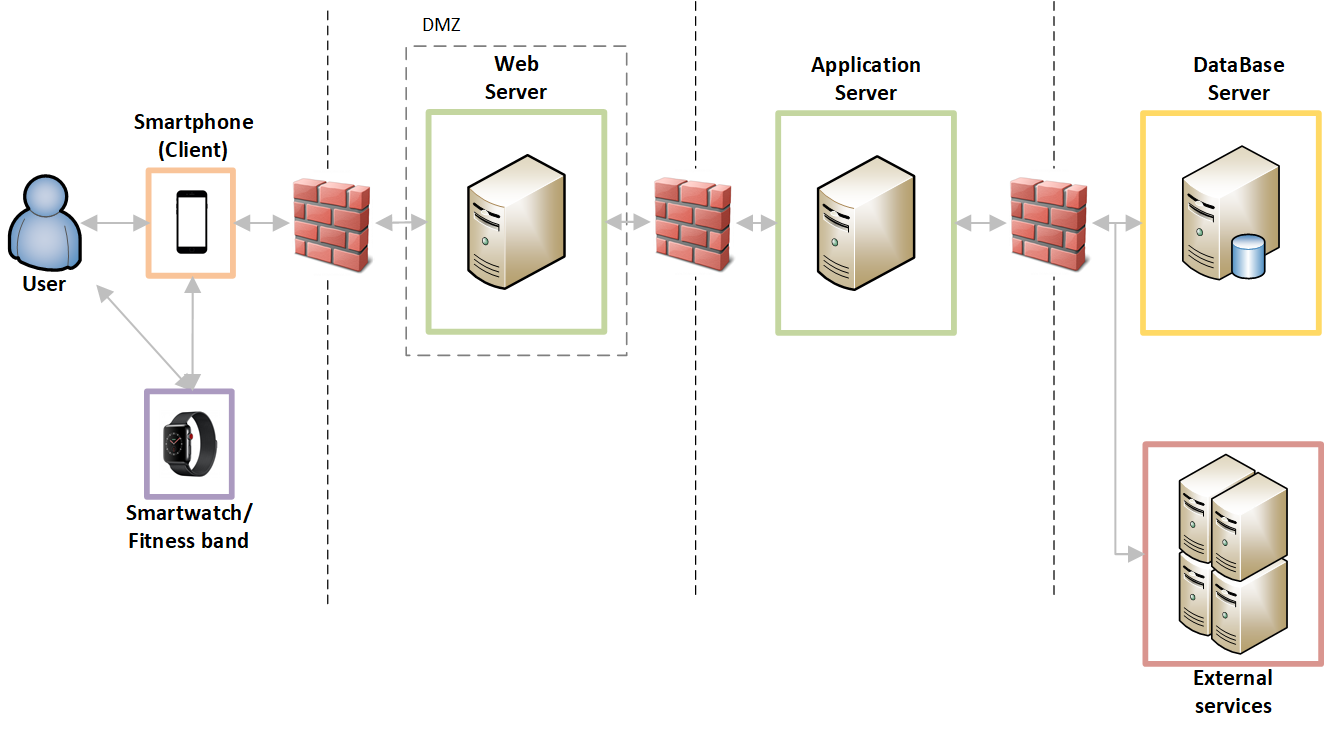
\includegraphics[scale=0.60]{pictures/Overview.png}}
    \caption{Overview of the system high level architecture}
    \label{fig:overview}
\end{figure}
\textbf{Figure \ref{fig:overview}} shows the high level architecture that the three applications will adopt.
They will be deployed in a 4-tier client-server architecture, composed by:
\begin{itemize}
    \item a distributed presentation layer on the Client, that also retrieves information from the smart-watch or fitness band;
    \item a Web Server for load balancing, failure detection, message filtering and forwarding;
    \item an Application Server that runs the business logic;
    \item a Database Server containing the applications' data.
\end{itemize}
They will also have to communicate with external services (Google Maps and an ambulance service). For further details on the 4-tier client-server architecture, refer to \textbf{section \ref{ArchitecturalStylesAndPatterns}}.

There are three firewalls among the four tiers, so as to guarantee a level of security as high as possible. The one between the Client and the Web Server filters all the requests coming from the former, allowing only a restricted amount of operations. 

The Web Server, however, is still considered to be in an untrustworthy zone (DMZ) because it is in close contact with the web and the (possibly malicious) Clients. Therefore, after the request is received and analysed by the Web Server, it is sent to the Application Server through a second firewall, that should guarantee that only well formed request are accepted. 

The last firewall is placed between the Application Server and the Database Server and it makes sure of the fact that only certain operations on the data can be performed by specific components (see \textbf{section \ref{RuntimeView}}).
This firewall also filters the messages exchanged with the external services.

All the firewalls work in the opposite direction too, allowing only those operation that the applications are built to offer.


